\begin{figure}[t]
\centering
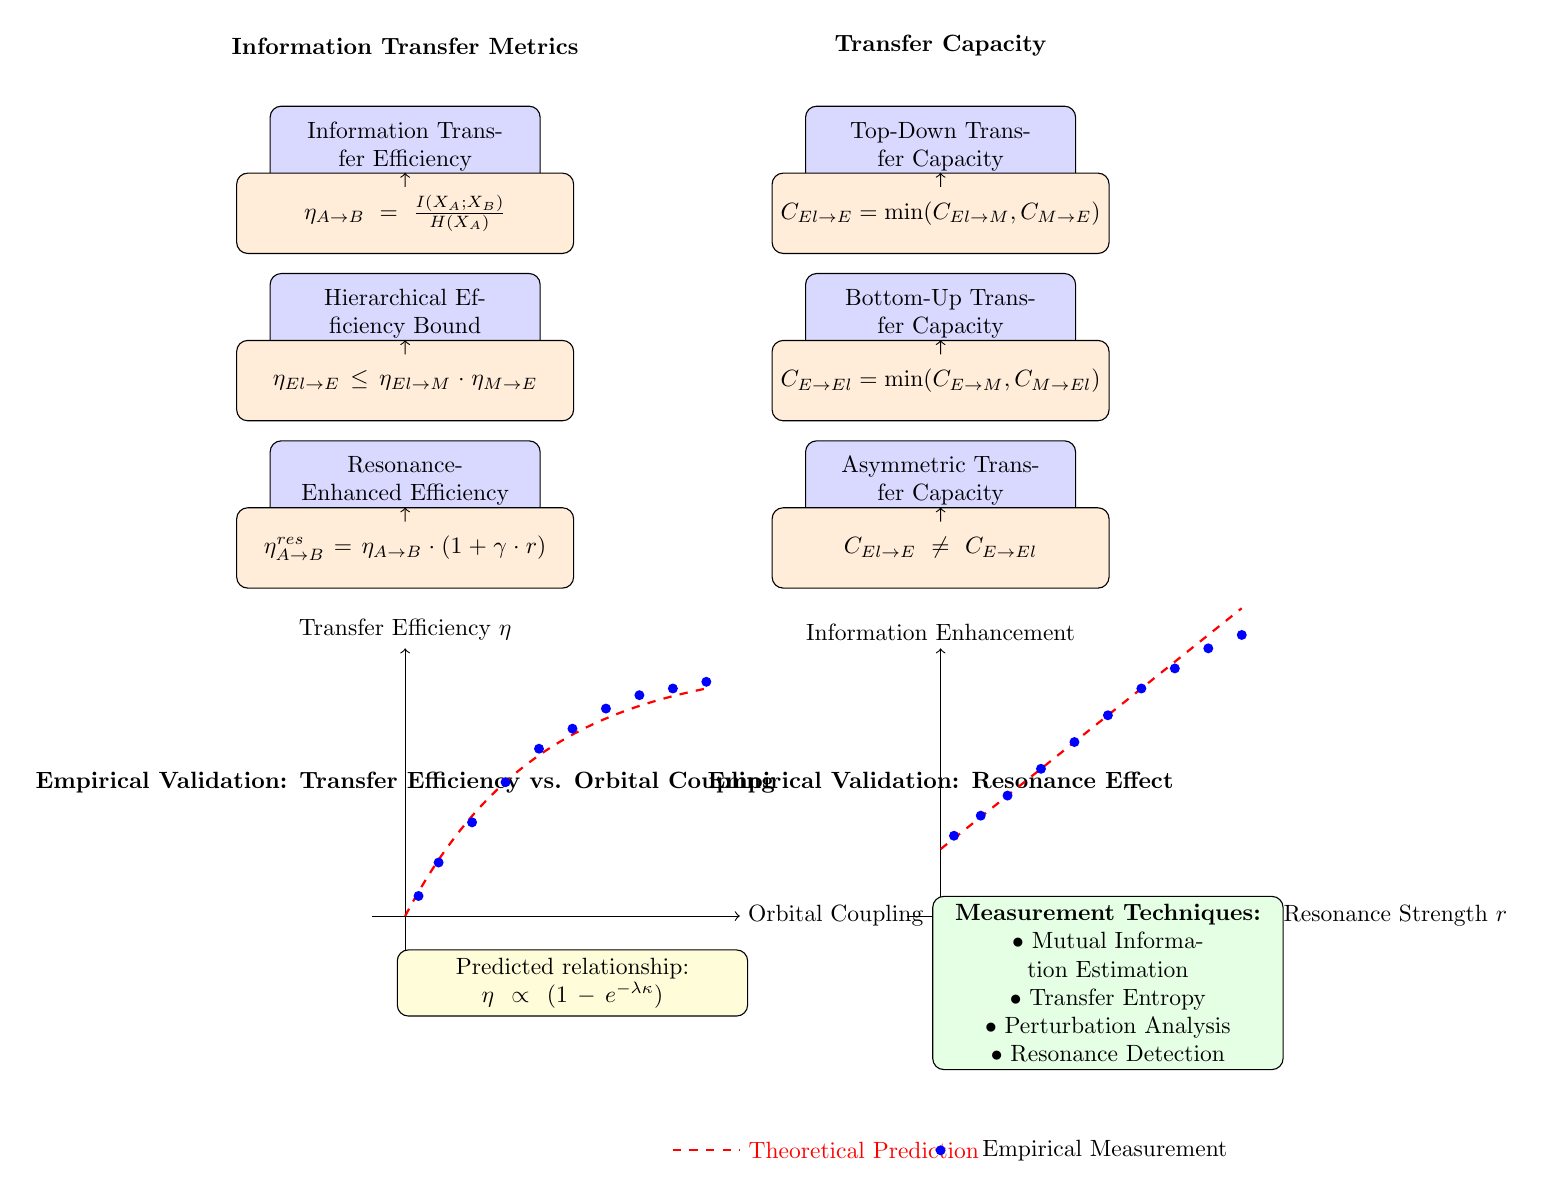
\begin{tikzpicture}[scale=0.85, transform shape]
    % Define styles
    \tikzset{
        metric/.style={
            draw,
            fill=blue!15,
            rounded corners,
            minimum width=4cm,
            minimum height=1.2cm,
            text width=3.8cm,
            align=center
        },
        equation/.style={
            draw,
            fill=orange!15,
            rounded corners,
            minimum width=5cm,
            minimum height=1.2cm,
            text width=4.8cm,
            align=center
        },
        point/.style={
            circle,
            fill=blue,
            inner sep=1.5pt
        },
        theory/.style={
            red,
            thick,
            dashed
        }
    }
    
    % Transfer efficiency metrics
    \begin{scope}[shift={(0,0)}]
        % Title
        \node[font=\bfseries] at (0,5) {Information Transfer Metrics};
        
        % Efficiency metric
        \node[metric] (eff) at (0,3.5) {Information Transfer Efficiency};
        \node[equation] (eff_eq) at (0,2.5) {
            $\eta_{A \to B} = \frac{I(X_A; X_B)}{H(X_A)}$
        };
        
        % Hierarchical efficiency bound
        \node[metric] (h_eff) at (0,1) {Hierarchical Efficiency Bound};
        \node[equation] (h_eff_eq) at (0,0) {
            $\eta_{El \to E} \leq \eta_{El \to M} \cdot \eta_{M \to E}$
        };
        
        % Resonance-enhanced efficiency
        \node[metric] (r_eff) at (0,-1.5) {Resonance-Enhanced Efficiency};
        \node[equation] (r_eff_eq) at (0,-2.5) {
            $\eta_{A \to B}^{res} = \eta_{A \to B} \cdot (1 + \gamma \cdot r)$
        };
        
        % Connect metrics to equations
        \draw[->] (eff) -- (eff_eq);
        \draw[->] (h_eff) -- (h_eff_eq);
        \draw[->] (r_eff) -- (r_eff_eq);
    \end{scope}
    
    % Transfer capacity measurements
    \begin{scope}[shift={(8,0)}]
        % Title
        \node[font=\bfseries] at (0,5) {Transfer Capacity};
        
        % Top-down capacity
        \node[metric] (td_cap) at (0,3.5) {Top-Down Transfer Capacity};
        \node[equation] (td_cap_eq) at (0,2.5) {
            $C_{El \to E} = \min(C_{El \to M}, C_{M \to E})$
        };
        
        % Bottom-up capacity
        \node[metric] (bu_cap) at (0,1) {Bottom-Up Transfer Capacity};
        \node[equation] (bu_cap_eq) at (0,0) {
            $C_{E \to El} = \min(C_{E \to M}, C_{M \to El})$
        };
        
        % Asymmetric capacity
        \node[metric] (asym_cap) at (0,-1.5) {Asymmetric Transfer Capacity};
        \node[equation] (asym_cap_eq) at (0,-2.5) {
            $C_{El \to E} \neq C_{E \to El}$
        };
        
        % Connect
        \draw[->] (td_cap) -- (td_cap_eq);
        \draw[->] (bu_cap) -- (bu_cap_eq);
        \draw[->] (asym_cap) -- (asym_cap_eq);
    \end{scope}
    
    % Empirical validation
    \begin{scope}[shift={(0,-8)}]
        % Title
        \node[font=\bfseries] at (0,2) {Empirical Validation: Transfer Efficiency vs. Orbital Coupling};
        
        % Axes
        \draw[->] (-0.5,0) -- (5,0) node[right] {Orbital Coupling $\kappa_{AB}$};
        \draw[->] (0,-0.5) -- (0,4) node[above] {Transfer Efficiency $\eta$};
        
        % Theoretical curve
        \draw[theory, domain=0:4.5, samples=100, smooth, variable=\x] 
            plot ({\x}, {3.8 * (1 - exp(-0.5*\x))});
        
        % Data points
        \foreach \x/\y in {0.2/0.3, 0.5/0.8, 1/1.4, 1.5/2.0, 2/2.5, 2.5/2.8, 3/3.1, 3.5/3.3, 4/3.4, 4.5/3.5}
            \node[point] at (\x,\y) {};
        
        % Predicted relationship
        \node[draw, fill=yellow!15, rounded corners, text width=5cm, align=center] at (2.5,-1) {
            Predicted relationship:\\
            $\eta \propto (1 - e^{-\lambda \kappa})$
        };
    \end{scope}
    
    % Resonance measurement
    \begin{scope}[shift={(8,-8)}]
        % Title
        \node[font=\bfseries] at (0,2) {Empirical Validation: Resonance Effect};
        
        % Axes
        \draw[->] (-0.5,0) -- (5,0) node[right] {Resonance Strength $r$};
        \draw[->] (0,-0.5) -- (0,4) node[above] {Information Enhancement};
        
        % Theoretical relationship
        \draw[theory, domain=0:4.5, samples=100, smooth, variable=\x] 
            plot ({\x}, {1 + 0.8*\x});
        
        % Data points
        \foreach \x/\y in {0.2/1.2, 0.6/1.5, 1/1.8, 1.5/2.2, 2/2.6, 2.5/3.0, 3/3.4, 3.5/3.7, 4/4.0, 4.5/4.2}
            \node[point] at (\x,\y) {};
        
        % Measurement techniques
        \node[draw, fill=green!10, rounded corners, text width=5cm, align=center] at (2.5,-1) {
            \textbf{Measurement Techniques:}\\
            $\bullet$ Mutual Information Estimation\\
            $\bullet$ Transfer Entropy\\
            $\bullet$ Perturbation Analysis\\
            $\bullet$ Resonance Detection
        };
    \end{scope}
    
    % Legend
    \begin{scope}[shift={(4,-11.5)}]
        \draw[theory] (0,0) -- (1,0) node[right] {Theoretical Prediction};
        \node[point] at (4,0) {};
        \node[right] at (4.5,0) {Empirical Measurement};
    \end{scope}
    
\end{tikzpicture}
\caption{Information transfer metrics and empirical validation. Top left: Key metrics for quantifying information transfer in the Elder system, including transfer efficiency $\eta_{A \to B} = \frac{I(X_A; X_B)}{H(X_A)}$, hierarchical efficiency bound $\eta_{El \to E} \leq \eta_{El \to M} \cdot \eta_{M \to E}$, and resonance-enhanced efficiency $\eta_{A \to B}^{res} = \eta_{A \to B} \cdot (1 + \gamma \cdot r)$. Top right: Transfer capacity measures including top-down capacity $C_{El \to E} = \min(C_{El \to M}, C_{M \to E})$, bottom-up capacity $C_{E \to El} = \min(C_{E \to M}, C_{M \to El})$, and the asymmetric nature of these capacities $C_{El \to E} \neq C_{E \to El}$. Bottom left: Empirical validation of transfer efficiency versus orbital coupling, showing that efficiency increases with coupling strength following the predicted relationship $\eta \propto (1 - e^{-\lambda \kappa})$. Bottom right: Empirical validation of resonance effect on information transfer, confirming the linear enhancement relationship $I_{res} = I \cdot (1 + \gamma \cdot r)$, with measurements obtained through techniques such as mutual information estimation, transfer entropy, perturbation analysis, and resonance detection.}
\label{fig:transfer_metrics}
\end{figure}